\documentclass[12pt]{jarticle}
\usepackage{graphicx}
\textwidth=16cm
\oddsidemargin=0cm

\newcommand \Br [1] {\left( #1 \right)}

\renewcommand  \[  {\begin{eqnarray}}
\renewcommand  \]  {\end{eqnarray}}

\begin{document}


\title{工学基礎実験実習 やさしいC言語\\最終レポート}
\date{出題日: 2019年7月9日 \\
      提出日: \today \\
      締切日: 2019年7月23日 \\} 
\author{氏名:重近大智\\学生番号:09501527}
\maketitle

\section{はじめに}
本レポートでは,ニュートン法を用いて,与えられた4つの課題を解く.まず,ニュートン法の計算を反復するC言語プログラムの作成方針を示す.次に,プログラムについて説明し,実験結果を示す.最後に考察とまとめを行う.一連のレポートは\LaTeX{}を用いて作成した.また,課題で与えられた関数に関する図,また,使用したC言語プログラムのソースはレポートの最後にまとめて表示する.

\section{プログラム作成方針}
まず,作成するC言語プログラムにおいて最も重要なのは,解の近似値を求めるニュートン法の計算を繰り返し実行することと,処理が終了しないのを防ぐために,適切な終了条件を設定することである.今回は課題1において3つの方程式の解の近似値を求める必要があるため,ニュートン法の式で登場する$f(x)$,$f\prime(x)$を別の関数として定義しておくことで,このC言語プログラムを$f(x)$に応じて,容易に書き換えられるようにしておくことが求められた.
\section{プログラムの説明}
まず,課題1を解くにあたって作成したC言語プログラムの内容について説明する.
\begin{itemize}
\item{7〜8行目:C言語プログラム内の関数を利用するのに必要となるヘッダを記述している.}
\item{10〜14行目:課題で与えられた$f(x)$を呼び出す関数を定義している.ニュートン法の計算の際に呼び出す.}
\item{16〜20行目:与えられた$f(x)$の1次導関数$f\prime(x)$を定義している.ニュートン法の計算の際に呼び出す.}
\item{22〜26行目:ニュートン法の計算を行う関数を定義している.ここで先述の2つの関数を呼び出す.}
\end{itemize}
\verb|main|関数は長くなっているため,分けて説明する.28〜50行目で\verb|main|関数を定義している.
\begin{itemize}
\item{31〜36行目:この後の計算で使用する整数(\verb|int|型),倍精度浮動小数点数(\verb|double|型)の初期値を設定する.この値には許容誤差と初期値の設定も含まれる.}
\item{38〜39行目:プログラムが起動したことを示す確認メッセージを表示する.}
\item{41〜42行目:$f(x_k)$の値が許容誤差よりも小さくなった場合に処理を終了する.終了しない場合は,43〜46行目の処理を繰り返す.}
\item{43行目:処理を実行した回数を数えるために使用される.整数値$n$に1を加えて,$n$をその値で置き換える.}
\item{44行目:ニュートン法の計算を行う関数を呼び出し,その計算結果で$x_k$を置き換える.}
\item{45行目:$n$,$x_k$,$f(x_k)$,$ans-x_k$の結果を表示する.}
\item{48〜49行目:処理が完了したことを示す確認メッセージを表示する.}
\end{itemize}
以上が課題1で用いたC言語プログラムの内容である.


続いて,課題2を解くにあたって作成したC言語プログラムで課題1のプログラムとは異なる動作をする部分を説明する.
\begin{itemize}
\item{44行目:表示内容が課題1のプログラムとは異なる.$k$,$x_k$,$f(x_k)$,$f\prime(x_k)$の結果を表示する.}
\end{itemize}
以上が課題1で用いたC言語プログラムと異なる動作をする部分である.
\section{実験}
\label{sec:exp}
C言語プログラムは「\verb|gcc -lm| [ファイル名.c]」でコンパイルを行い,「\verb|./a.out|」で実行した.
\subsection{課題1}
課題1で与えられた方程式は次の3つである.
\begin{equation}
f(x)=\sin e^x = 0
\label{eq:1-am}
\end{equation}
\begin{equation}
f(x)=x^3-3x-2 = 0
\label{eq:1-bm}
\end{equation}
\begin{equation}
f(x)=x^3-x^2-x+1 = 0
\label{eq:1-cm}
\end{equation}
まず,1つ目の方程式(式\ref{eq:1-am})について考える.方程式の解は,$f(x)=\sin\pi=0$
と考えると,$e^x=\pi$となるから,$x=\log\pi$が解である.C言語プログラム内の真の解の値には$\log\pi$を入力した.
導関数は$f\prime(x)=e^x\cos e^x$であるから,ニュートン法の反復式は次のようになる.
\[
\label{eq:1-a}
x_{k+1}=x_k- \frac{\sin e^{x_k}}{e^{x_k}\cos e^{x_k}}
\]
初期値$x_0$を$1$とし,C言語プログラムで式\ref{eq:1-a}の反復計算を行った.結果を表\ref{tab:1-a}に示す.
\begin{table}[t]
 \caption{1つ目の方程式に関する反復回数$k$,求められた解の近似値$x_k$,$f(x_k)$,真の解との誤差\textbar $x_k-a$\textbar}
 \label{tab:1-a}
 \center
\begin{tabular}{|c|c|c|c|}
\hline
 $k$ & $xk$ & $f(xk)$ & $xk-a$\\
\hline
1  & 1.1657479108 & -0.0666793608 & 0.0210180250\\
2  & 1.1449182997 & -0.0005919752 & 0.0001884138\\
3  & 1.1447299036 & -0.0000000557 & 0.0000000177\\
4  & 1.1447298858 & -0.0000000000 & 0.0000000000\\
5  & 1.1447298858 & 0.0000000000 & 0.0000000000\\
\hline
 \end{tabular}
\end{table}


次に,2つ目の方程式(式\ref{eq:1-bm})について考える.方程式の解は,$f(x)=x^3-3x-2=0$と考えると,$x=-1$が解の1つとなる.C言語プログラム内の真の解の値には$-1$を入力した.
導関数は$f\prime(x)=3x^2-3$であるから,ニュートン法の反復式は次のようになる.
\[
\label{eq:1-b}
x_{k+1}=x_k- \frac{x_k^3-3x_k-2}{3x_k^2-3}
\]
初期値$x_0$を$-8$とし,C言語プログラムで式\ref{eq:1-b}の反復計算を行った.結果を表\ref{tab:1-b}に示す.ただし,収束するまで回数を要したため,最後の5回のみを表示する.
\begin{table}[t]
 \caption{2つ目の方程式に関する反復回数$k$,求められた解の近似値$x_k$,$f(x_k)$,真の解との誤差\textbar $x_k-a$\textbar}
 \label{tab:1-b}
 \center
\begin{tabular}{|c|c|c|c|}
\hline
$k$ & $xk$ & $f(xk)$ & $xk-a$\\
\hline
28  & -1.0000000712 & -0.0000000000 & 0.0000000712\\
29  & -1.0000000349 & -0.0000000000 & 0.0000000349\\
30  & -1.0000000189 & -0.0000000000 & 0.0000000189\\
31  & -1.0000000111 & -0.0000000000 & 0.0000000111\\
32  & -1.0000000045 & 0.0000000000 & 0.0000000045\\
\hline
 \end{tabular}
\end{table}


次に,3つ目の方程式(式\ref{eq:1-cm})について考える.方程式の解は,$f(x)=x^3-x^2-x+1=0$
と考えると,$x=1$が解の1つとなる.C言語プログラム内の真の解の値には$1$を入力した.導関数は$f\prime(x)=3x^2-2x-1$であるから,ニュートン法の反復式は次のようになる.
\[
\label{eq:1-c}
x_{k+1}=x_k- \frac{x_k^3-x_k^2-x_k+1}{3x_k^2-2x_k-1}
\]
初期値$x_0$を$6$とし,C言語プログラムで式\ref{eq:1-c}の反復計算を行った.結果を表\ref{tab:1-c}に示す.ただし,収束するまで回数を要したため,最後の5回のみを表示する.
\begin{table}[t]
 \caption{3つ目の方程式に関する反復回数$k$,求められた解の近似値$x_k$,$f(x_k)$,真の解との誤差\textbar $x_k-a$\textbar}
 \label{tab:1-c}
 \center
\begin{tabular}{|c|c|c|c|}
\hline
$k$ & $xk$ & $f(xk)$ & $xk-a$ \\
\hline
27  & 1.0000001053 & 0.0000000000 & 0.0000001053\\
28  & 1.0000000527 & 0.0000000000 & 0.0000000527\\
29  & 1.0000000263 & 0.0000000000 & 0.0000000263\\
30  & 1.0000000132 & 0.0000000000 & 0.0000000132\\
31  & 1.0000000066 & 0.0000000000 & 0.0000000066\\
\hline
 \end{tabular}
\end{table}

\subsection{課題2}
課題2で与えられた方程式は次のとおりである.
\[
f(x)=x^3-2x-5 = 0
\label{eq:2m}
\]
この方程式(式\ref{eq:2m})について考える.導関数は,$f\prime(x)=3x^2-2$であるから,ニュートン法の反復式は次のようになる.
\[
x_{k+1}=x_k- \frac{x_k^3-2x_k-5}{3x_k^2-2}
\label{eq:2}
\]
課題1とは異なり,初期値$x_0$は$0$と決められている.また,収束の様子を詳しく調べるため,$k$,$x_k$,$f(x_k)$,および$f\prime(x_k)$の値を表示する.このために,課題1とは異なるC言語プログラムを使用した.その結果を表\ref{tab:2}に示す.
\begin{table}[t]
\caption{課題2の反復回数$k$,解の近似値$x_k$,$f(x_k)$,$f\prime(x_k)$}
\label{tab:2}
\center
\begin{tabular}{|c|c|c|c|}
\hline
$k$ & $xk$ & $f(xk)$ & $f'(xk)$\\
\hline
1 & -2.500000 & -15.625000 & 16.750000 \\
2 & -1.567164 & -5.714632 & 5.368011 \\
3 & -0.502592 & -4.121770 & -1.242203 \\
4 & -3.820706 & -53.132488 & 41.793394 \\
5 & -2.549393 & -16.470758 & 17.498220 \\
6 & -1.608111 & -5.942390 & 5.758068 \\
7 & -0.576100 & -4.039002 & -1.004325 \\
8 & -4.597710 & -92.995258 & 61.416800 \\
9 & -3.083543 & -28.151977 & 26.524715 \\
10 & -2.022194 & -9.224909 & 10.267809 \\
11 & -1.123764 & -4.171613 & 1.788537 \\
12 & 1.208652 & -5.651658 & 2.382516 \\
13 & 3.580790 & 33.751515 & 36.466172 \\
14 & 2.655233 & 8.409627 & 19.150790 \\
15 & 2.216106 & 1.451367 & 12.733381 \\
16 & 2.102125 & 0.084892 & 11.256789 \\
17 & 2.094584 & 0.000358 & 11.161841 \\
18 & 2.094551 & 0.000000 & 11.161438 \\
19 & 2.094551 & -0.000000 & 11.161438 \\
\hline
\end{tabular}
\end{table}
\section{プログラムの作成に関する考察}
課題1の方程式の解の近似値をC言語プログラムを用いて求めるとき,初期値によっては他の解に近付くことがあった.解が複数ある方程式の解を求めるときは,注意する必要がある.課題1の一部の方程式では,小数点以下の数字が全て$0$となっているにも関わらず,処理が数回続く場合があった.この問題は,小数点以下の表示桁数を$10$桁にすることで解決した(実際には処理は進んでいた).
また,課題2では,許容誤差を$3E-16$にしていると,計算が終了しなかった.計算機の計算精度の限界により,収束条件を満たさなかったと考えられる.
\section{まとめ}
ニュートン法を用いたC言語プログラムで,与えられた課題の方程式の解の近似値を求めることができた.表\ref{tab:1-a}の結果より式\ref{eq:1-am}に関するニュートン法の計算はすぐに収束することが分かったが,なぜ式\ref{eq:1-bm},\ref{eq:1-cm}に関するニュートン法の計算はすぐには収束しなかったのだろうか.これについては更なる検討を必要とする.
\section{課題で出題された関数の図}
関数の図は次のページに表示する.
\begin{figure}[p]
\begin{minipage}{7.95cm}
\center
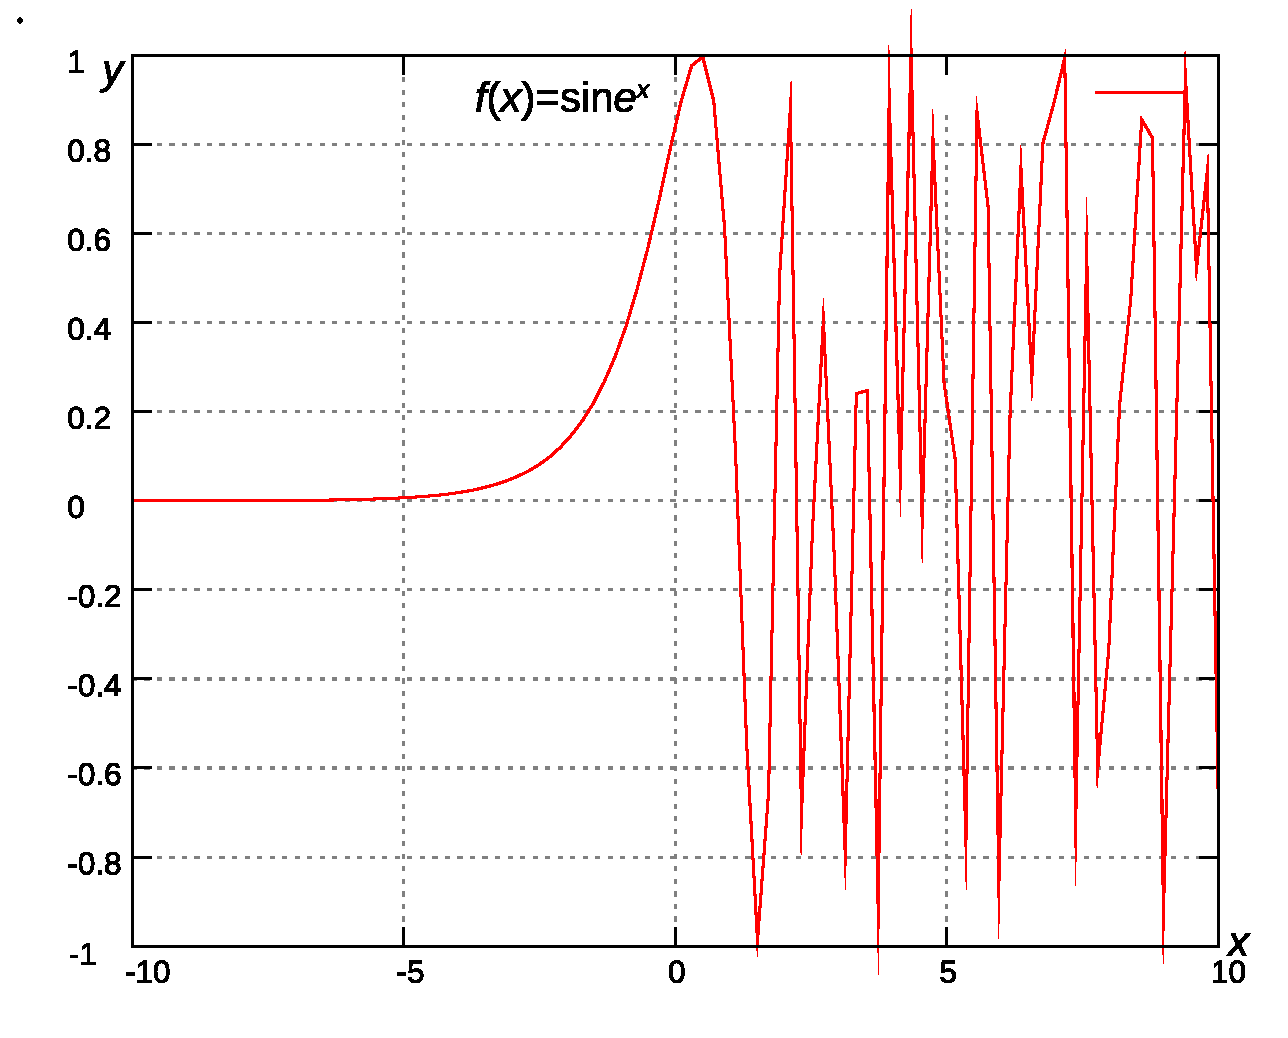
\includegraphics[scale=0.38]{graph1a.eps}
\caption{式\ref{eq:1-am}の図}
\label{fig:1-am}
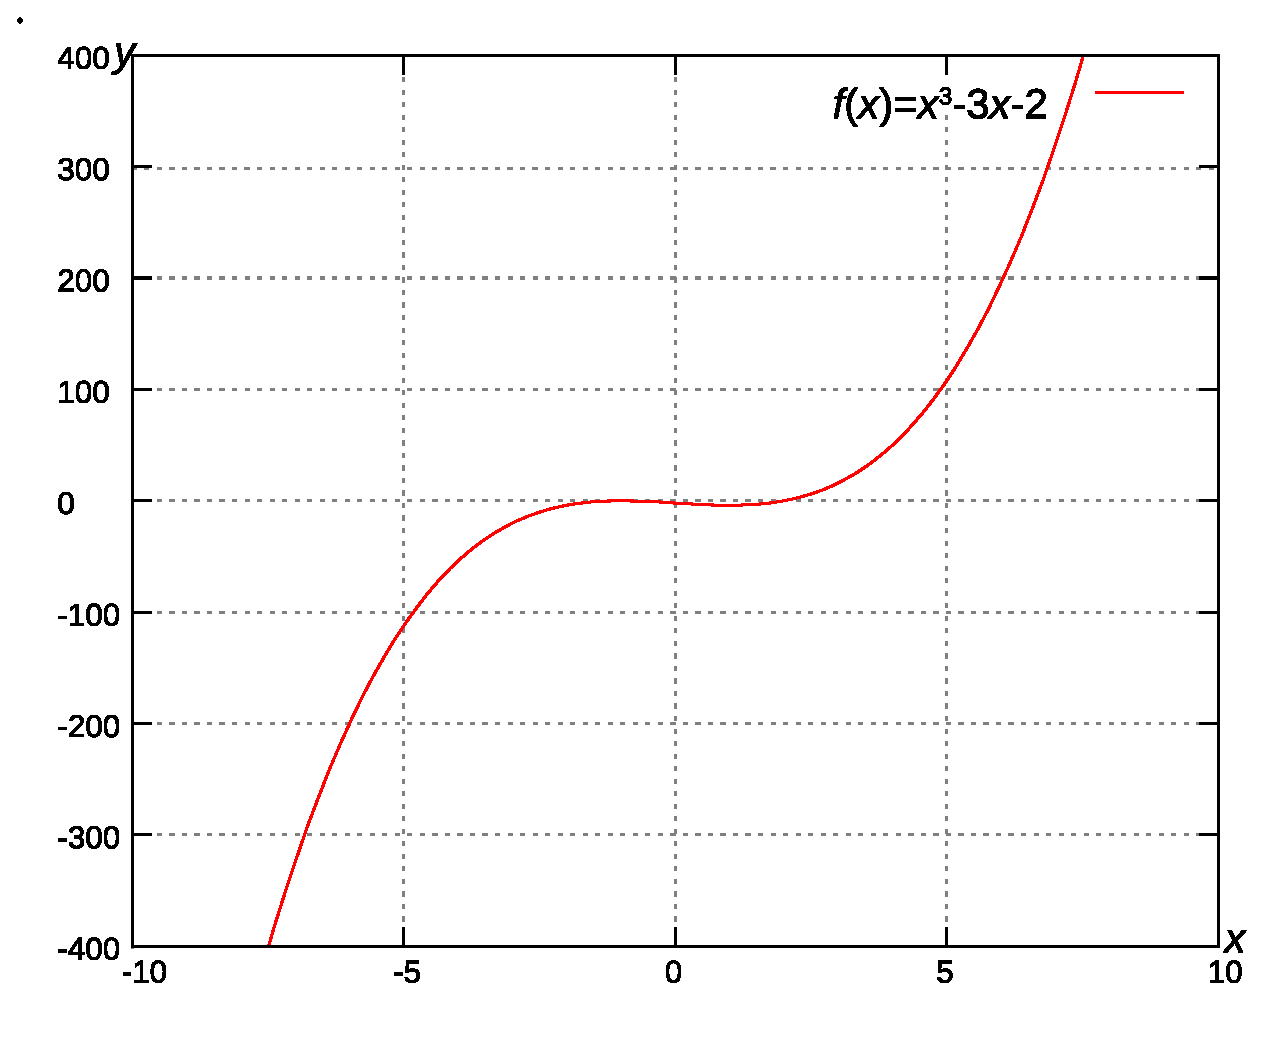
\includegraphics[scale=0.38]{graph2.eps}
\caption{式\ref{eq:1-bm}の図}
\label{fig:1-bm}
\end{minipage}
\begin{minipage}{7.95cm}
\center
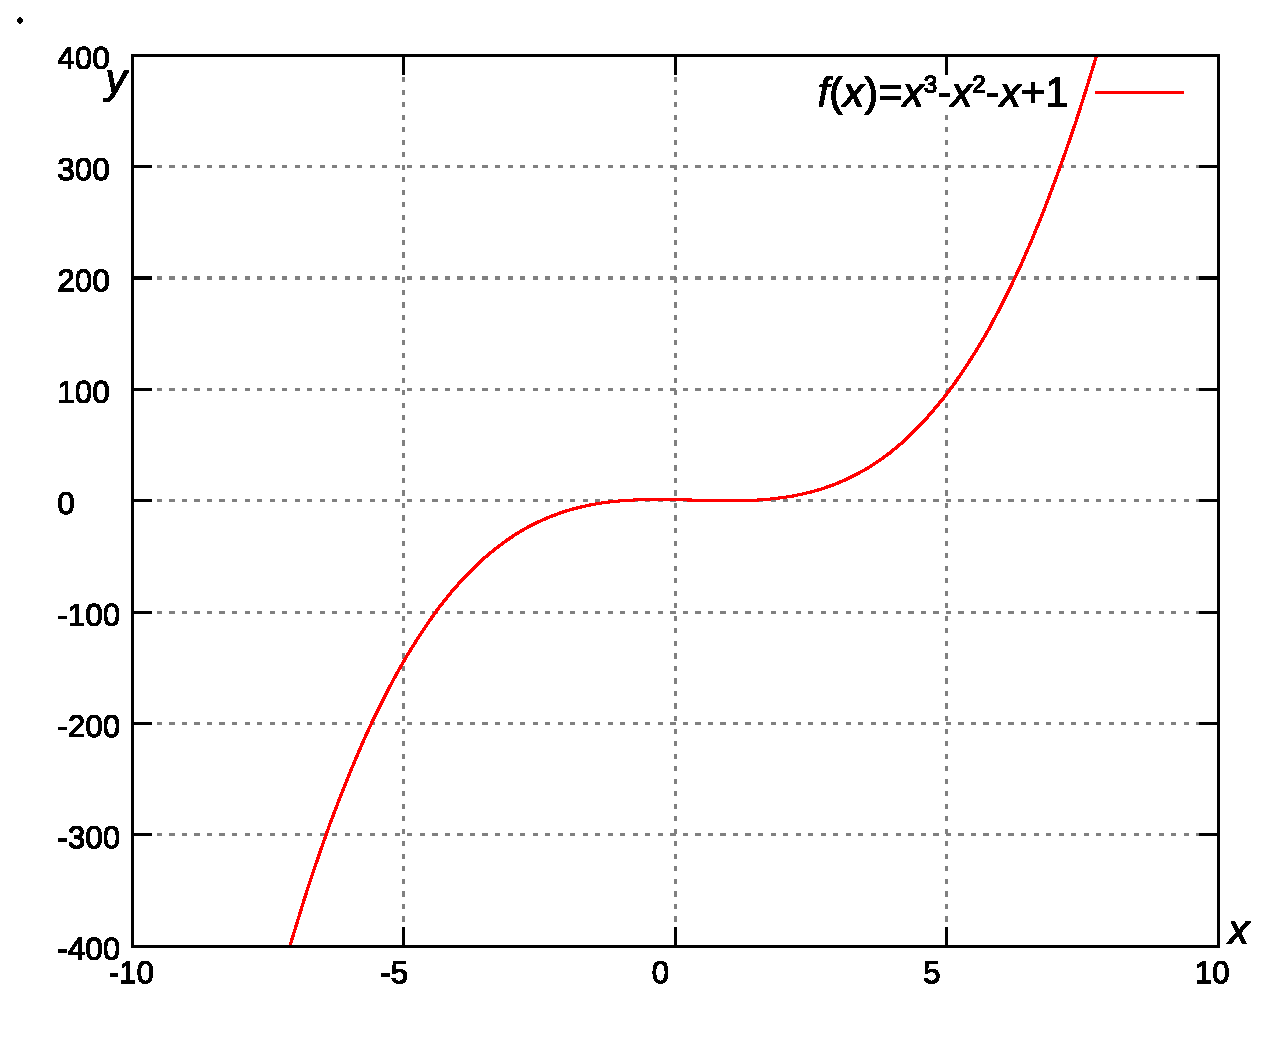
\includegraphics[scale=0.38]{graph3.eps}
\caption{式\ref{eq:1-cm}の図}
\label{fig:1-cm}
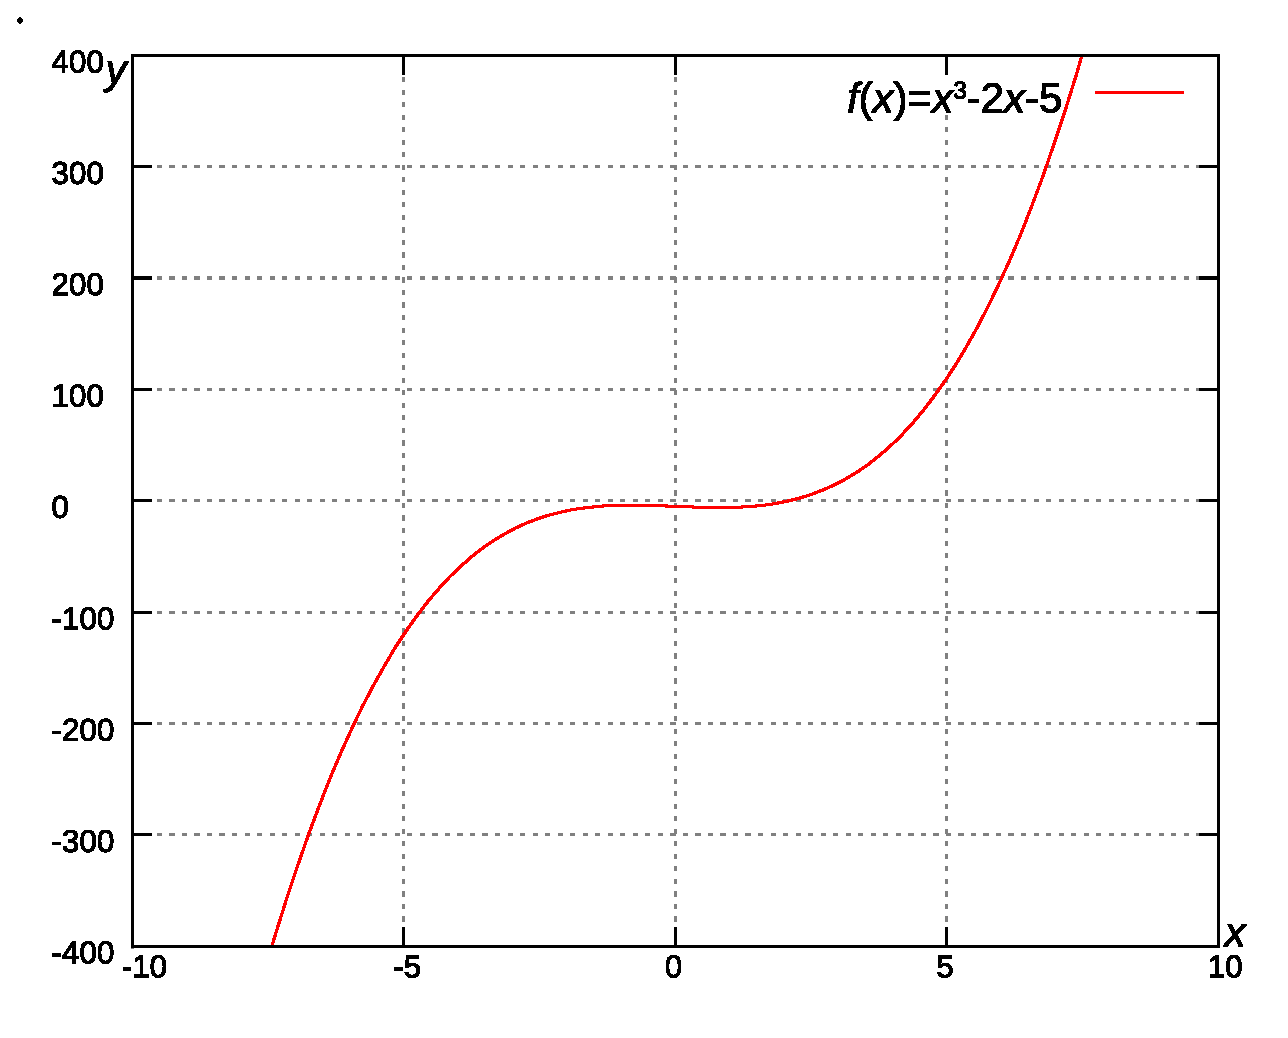
\includegraphics[scale=0.38]{graph4.eps}
\caption{式\ref{eq:2m}の図}
\label{fig:2-m}
\end{minipage}
\end{figure}

\section{C言語プログラムのソース}
課題1で用いたプログラムのソース(50行) \\
これは,式\ref{eq:1-a}の反復計算に用いたプログラムだが,式\ref{eq:1-b},\ref{eq:1-c}の計算では,元の関数,導関数,初期値を変更して使用した.
\begin{verbatim}
     1	/*
     2	  ニュートン法による方程式の解法
     3	
     4	  コンパイル方法:gcc 1-a.c
     5	*/
     6	
     7	#include <stdio.h>  /*printfを利用するのに必要*/
     8	#include <math.h>   /*各種算術関数のために必要*/
     9	
    10	/* f(x) = 0 の x を求める問題となる関数 */
    11	double f(double x)
    12	{
    13	    return sin(exp(x));
    14	}
    15	
    16	/* f の一次導関数*/
    17	double f1(double x)
    18	{
    19	    return exp(x) * cos(exp(x));
    20	}
    21	
    22	/* ニュートン法の繰り返し関数 */
    23	double newton(double xk)
    24	{
    25	    return xk - (f(xk) / f1(xk));
    26	}
    27	
    28	main()
    29	{
    30	
    31	    /* 各種初期値設定 */
    32	    int n = 0;                                                                         
 /* 繰り返し回数の初期値 */
    33	    double ans = log(3.1415926535897932384626433832795028841971
6939937510582097494459); /* 真のx */
    34	    double delta = 3E-16;                                                              
 /* 許容誤差3E-16 */
    35	
    36	    double xk = 1;                                                                     
 /* 初期値 */
    37	
    38	    /* 開始メッセージを表示 */
    39	    printf("Newton method program start.\n");
    40	
    41	    /* fabs(x) … x の絶対値を求める関数*/
    42	    while(fabs(f(xk)) > delta){ /* 収束条件:f(x) がdelta以下になる */
    43	        n = n + 1;
    44	        xk = newton(xk);
    45	        printf("n:%d xk:%.10f f(xk):%.10f ans-xk:%.10f\n", n, xk,
 f(xk), ans - xk);
    46	    }
    47	
    48	    /* 終了メッセージを表示 */
    49	    printf("done.\n");
    50	}
\end{verbatim}
課題2で用いたプログラムのソース(49行)
\begin{verbatim}
     1	/*
     2	  ニュートン法による方程式の解法
     3	
     4	  コンパイル方法:gcc -lm 2.c
     5	*/
     6	
     7	#include <stdio.h>  /*printfを利用するのに必要*/
     8	#include <math.h>   /*各種算術関数のために必要*/
     9	
    10	/* f(x) = 0 の x を求める問題となる関数 */
    11	double f(double x)
    12	{
    13	    return x * x * x - 2 * x - 5;
    14	}
    15	
    16	/* f の一次導関数*/
    17	double f1(double x)
    18	{
    19	    return 3 * x * x - 2;
    20	}
    21	
    22	/* ニュートン法の繰り返し関数 */
    23	double newton(double xk)
    24	{
    25	    return xk - (f(xk) / f1(xk));
    26	}
    27	
    28	main()
    29	{
    30	
    31	    /* 各種初期値設定 */
    32	    int n = 0;            /* 繰り返し回数の初期値 */
    33	    double delta = 3E-15; /* 許容誤差3E-15 */
    34	
    35	    double xk = 0;        /* 初期値 */
    36	
    37	    /* 開始メッセージを表示 */
    38	    printf("Newton method program start.\n");
    39	
    40	    /* fabs(x) … x の絶対値を求める関数*/
    41	    while(fabs(f(xk)) > delta){ /* 収束条件:f(x) がdelta以下になる */
    42	        n = n + 1;
    43	        xk = newton(xk);
    44	        printf("k:%d xk:%f f(xk):%f f'(xk):%f\n", n, xk, f(xk),
 f1(xk));
    45	    }
    46	
    47	    /* 終了メッセージを表示 */
    48	    printf("done.\n");
    49	}
\end{verbatim}
\end{document}
